% Framside til eksamen (HBV-mal)
% S.G. 15/52014.
% C.T. 2015-11-20
% C.T. 2016-02-01

\documentclass[noanswers,12pt]{exam}	% Documentclass exam har mulighet for å slå av og på solution områdene i utfila
\usepackage[a4paper,left=2.3cm,top=2.9cm,right=2.2cm,bottom=2.9cm,includefoot]{geometry}
%\usepackage{fancyhdr}
\usepackage[utf8]{inputenc} 
\usepackage{amsmath, amsthm, amssymb, amsfonts}
\usepackage{pgf}
\usepackage{pgfplots}
\usepackage{tikz}
\usetikzlibrary{scopes}
\usetikzlibrary{calc}				% kun for beregning av % uttelling for hver deloppgave 
\usepgfplotslibrary{fillbetween}
\usepackage{tkz-euclide}
\usetkzobj{all}
\usepackage{lastpage}
\usepackage{multirow}
\usepackage{hhline}
\usepackage{tabularx}
\usepackage{siunitx}
\usepackage{pgfplotstable}
\usepackage{ulem}

\newcommand{\ivec}{\mathbf{\hat{i}}}
\newcommand{\jvec}{\mathbf{\hat{j}}}

\newcommand{\diffd}{\mathop{}\!\mathrm{d}}
\newcommand{\diff}[2]{\frac{\diffd #1}{\diffd #2}}


\title{\vspace{-5cm}
	\author{}
	\date{}}


% INFO: Opplysningene i toppen på forsiden legges inn her:

\newcommand{\exsubjectcode}{MM-MAT4001}
\newcommand{\exsubjectname}{Mathematics}
\newcommand{\exdate}{Feb 25 2015}
\newcommand{\extime}{09:00-13:00}
\newcommand{\exhours}{4}
\newcommand{\exteacher}{Christian Bjørge Thoresen}
\newcommand{\excampus}{Vestfold}
\newcommand{\exfaculty}{TekMar}
\newcommand{\exassignments}{\numquestions}
\newcommand{\exattachments}{1}
\newcommand{\expages}{\numpages}



%\qformat{\textbf{Problem \thequestion: \thequestiontitle}\hfill}
\qformat{\Large{\textbf{Problem \thequestion}}\hfill}

\begin{document}
	\newgeometry{top = 2.5cm, bottom=1.5cm, left=1.5cm, right=1.5cm,includefoot}
	\maketitle
	\normalsize
	\thispagestyle{empty}    % Fjernar sidetal på framsida 
	%\fontfamily{phv}\selectfont 
		{\sffamily
		\noindent
		%\begin{tabular}{lp{15cm}}
%			  &
			%\raisebox{1.5cm}{
			\noindent
				\begin{tabularx}{\textwidth}{lX}
					%\begin{minipage}{0.7\textwidth} 
					\includegraphics[height=1.16cm]{figs/HSN_logo_en.pdf} & 
						\hfill \raisebox{1.3cm}{\small{ENGLISH} }  \vspace{0.2cm}     \\
					%\end{minipage}
				\end{tabularx}
					
					%\\
					\centering
					\Large{\bf \textsf{EXAMINATION INFORMATION PAGE} }    \\
					\large{\bf \textsf{Written examination} }            \\
				
		
		%\end{tabular}
		
		\vspace{1cm}
		\setlength{\extrarowheight}{2pt}
		
		\noindent
		\begin{tabularx}{\textwidth}{||X | X| X||}
			\hhline{|t:===:t|}
			Subject code: & \multicolumn{2}{l||}{ Subject name:}    \\ 
			\textbf{\exsubjectcode}     & \multicolumn{2}{l||}{ \exsubjectname}    \\ 
			\hhline{||---||}
			Examination date:               & Examination time from/to:  &  Total hours:       \\
			\exdate & \extime & \exhours \\
			\hhline{||---||}
			\multicolumn{3}{||l||}{Responsible subject teacher: }         \\
			\multicolumn{3}{||l||}{\exteacher }         \\
			\hhline{||---||}
			Campus:  & \multicolumn{2}{l||}{ Faculty:}    \\ 
			\excampus  & \multicolumn{2}{l||}{ \exfaculty}    \\ 
			\hhline{|:===:|}
			No. of assignments:    & No. of attachments:  & No. of pages incl. front     \\
			\exassignments & \exattachments & page and attachments: \expages       \\
			\hhline{||---||}
		\end{tabularx}
		
		% Calculation of the percent score for each sub-assignment - problem with tabularx on the first run when \numparts is undefined if it is put directly in there
		\ifdefined\numparts 
		\pgfmathparse{100/\numparts}
		\else
		\pgfmathparse{0}
		\fi
		
		\vspace{-1.5pt}
		\noindent
		\begin{tabularx}{\textwidth}{||X||}		%INFO: Tabellen for hjelpemilder, info om vedlegg og kommentarer er her
			\hhline{|:-:|}
			Permitted aids: \\
			Approved calculator: Citizen SR-270x and/or Casio fx-82ES PLUS \\[2.5cm]
			\hhline{||-||}
			Information regarding attachments: \\
			Formula sheet
			\\[2.5cm]
			\hhline{||-||}
			Comments: \\
			\sffamily{Each of the \numparts\ sub-assignment (a,b,c...) is weighted equally. Each counts \num[round-mode = figures, round-precision = 3,detect-all=true]{\pgfmathresult} \% towards the total score. }
			\\[2cm]
			\hhline{|b:=:b|}
		\end{tabularx}
		\vspace{0.5cm}
		
		\noindent
		\begin{tabularx}{\textwidth}{|X X X|}	
			\hline 
			\multicolumn{3}{|l|}{Select the type of examination paper } \\
			
			\textbf{Spreadsheets} & Line sheets & Blank sheets   \\ %INFO: Valg av papirtype her
			\hline 
		\end{tabularx}
		
		\vspace{0.5cm}
		\noindent
		\footnotesize{CANDIDATES MUST THEMSELVES CHECK THAT ALL ASSIGNMENTS AND ATTACHMENTS ARE IN ORDER
		}
		\normalsize
		
	}%\rmfamily
	\restoregeometry
	\pagebreak
	
	
% ---=== Slutt på forside ===---
	
	
	\begin{questions}
		
		\question
		\begin{parts}
%			\part Plot the function 
%			\[f(x) = \frac{x}{2} - 2, \quad -2 \leq x \leq 6 \]
%			
%			\begin{solution}
%				This is a straight line. We can calculate two points, or just use the vertical intercept and gradient to draw the line.
%				\begin{center}
%					\begin{tikzpicture}
%					\pgfplotsset{compat=1.12}
%					\begin{axis}[xmin=-2.5, xmax=6.5, ymin=-4.5, ymax=2.5, xlabel={$x$}, ylabel={$y$}, axis lines = middle, samples=100]
%					% use TeX as calculator:
%					\addplot[domain=-2:6,no markers]{x/2-2};
%					
%					\end{axis}
%					\end{tikzpicture}
%				\end{center}
%			\end{solution}
			
			\part Solve the set of equations and test the solution
			\begin{align*}
				3x - 9y &= 6\\
				2x + 5y &= 26
			\end{align*}
			%x = 8, y = 2 
			
			\begin{solution}
				\begin{align*}
					3x -9y &= 6\\
					3x &= 6 + 9y\\
					x &= \frac{6+9y}{3}\\
					x &= 2 + 3y\\
					\\
					2x + 5y &= 26\\
					2\left(2 + 3y\right) + 5y &= 26\\
					4 + 6y + 5y &= 26\\
					6y + 5y &= 26-4\\
					11y &= 22\\
					y &= 2\\
					\\
					x &= 2 + 3 y\\
					x &= 2 + 3 \cdot 2\\
					x &= 2 + 6\\
					x &= 8\\
				\end{align*}
				Final solution is \uuline{$x=8$ and $y=2$.}
				
				Left side eq1: $3\cdot 8 - 9 \cdot 2 = 24 - 18 = 6$
				
				Left side eq2: $2\cdot 8 + 5 \cdot 2 = 16 + 10 = 26$
				
				Our test shows that the solution is correct.
			\end{solution}
			
			\part Solve the inequality so that $x$ is on the left side in the solution
			\[2-4x < 2x+8\]
			
			\begin{solution}
				\begin{align*}
					2-4x &< 2x+8\\
					-4x - 2x &< 8 - 2\\
					-6x &< 6\\
					-x &< 1\\
					&\hspace*{-7pt}\underline{\underline{x > -1}}
				\end{align*}
			\end{solution}
			
			\part Solve the equation and test the solution
			\[5^{2x} = 125 \cdot 5^x\]
			
			\begin{solution}
				\begin{align*}
					5^{2x} &= 125 \cdot 5^x\\
					\frac{5^{2x}}{5^x} &= \frac{125 \cdot e^x}{e^x}\\
					5^{x} &= 125\\
					\ln 5^{x} &= \ln 125\\
					x\ln 5 &= \ln 125\\
					x &= \frac{\ln 125}{\ln 5}\\
					&\hspace*{-7pt}\uuline{x = 3}
				\end{align*}
				Testing solution
				
				Left side: $5^{2\cdot3} = 5^6 = 15625$
				
				Right side: $125 \cdot 5^3 = 125 \cdot 125 = 15625$
				
				The solution is correct.
			\end{solution}
			
%			\part Find the first derivative of
%			\[f(x) = 2x^3 + \sin 2x\]
%			
%			\begin{solution}
%				\begin{align*}
%					f'(x) &= 2\cdot 3x^2 + 2\cos 2x\\
%					f'(x) &= 6x^2 + 2\cos 2x\\
%				\end{align*}
%			\end{solution}
			
			\part Find the first derivative of
			\[f(x) = 2x^2\ln x\]
			
			\begin{solution}
				Using product rule:
				\begin{align*}
					u&=2x^2 \Rightarrow u' = 4x\\
					v&=\ln x \Rightarrow v' = \frac{1}{x}\\
					f'(x) &= u'v + v'u \\
					f'(x) &= 4x \cdot \ln x + \frac{1}{x} 2x^2 \\
					&\hspace*{-24pt}\uuline{f'(x) = 4x \ln x + 2x = 2x \left(2 \ln x + 1\right)}
				\end{align*}
			\end{solution}
			
			\part Find the first derivative of
			\[f(x) = \left(x^2+3\right)^5\]
			\begin{solution}
				Use the chain rule:
				\begin{align*}
					y(z) &= z^5 \Rightarrow \diff{y}{z} = 5z^4\\
					z(x)&=x^2+3 \Rightarrow \diff{z}{x} = 2x\\
					f(x) &= y(z)\\
					f'(x) &= \diff{y}{z} \diff{z}{x} \\
					f'(x) &= 5z^4 \cdot 2x\\
					&\hspace*{-24pt}\uuline{f'(x) = 10x\left(x^2+3\right)^4 }
				\end{align*}
			\end{solution}
			
			\part Find the indefinite integral
			\[\int 3x^2 \sin \left(x^3 + 3\right) \diffd x\]
			
			\begin{solution}
				Using substitution:
				\begin{align*}
					u &= x^3+3 \Rightarrow \diff{u}{x} = 3x^2 \Rightarrow \diffd x = \frac{\diffd u}{3x^2}\\
					\int 3x^2 \sin \left(x^3+3\right) \diffd x &= \int 3x^2 \sin u \frac{\diffd u}{3x^2}\\
					&= \int  \sin u \diffd u\\
					&= -\cos u + c\\
					&= \uuline{-\cos \left(x^3 + 3\right) + c}\\
				\end{align*}
			\end{solution}
			
			\part Find the indefinite integral
			\[\int 5x \sin x \diffd x\]
			
			\begin{solution}
				Integration by parts: 
				\begin{align*}
					u&=5x \Rightarrow u' = 5\\
					v'&=\sin x \Rightarrow  v = -\cos x\\
					\int 5x \sin x \diffd x &= \int u v' \diffd x\\
					&= uv - \int u' v \diffd x\\
					&= 5x \cdot \left(- \cos x \right) - \int 5 \left(-\cos x\right) \diffd x\\
					&=-5x\cos x + \int 5\cos x \diffd x\\
					&= \uuline{-5x\cos x + 5\sin x + c}\\
				\end{align*}
			\end{solution}
			
%			\part Find the definite integral
%			\[\int_0^1 1 \diffd x\]
			
%			\begin{solution}
%				\begin{align*}
%					\int_0^1 1 \diffd x &= \left[x\right]_0^1 = 1-0 = \uuline{1}
%				\end{align*}
%				
%			\end{solution}
			
		\end{parts}
		\newpage
		\question
		Given the function
		\[f\left(x\right) =  x^2 -2x - 3, \qquad -2 < x < 4 \]
		%(x-3)x(x+1)
%		is plotted below:
%		

		
		\begin{parts}

			
			\part Find the first and second derivative of $f(x)$, that is $\diff{f}{x}$ and $\diff{^2 f}{x^2}$.
			\begin{solution}
				\begin{align*}
					&\hspace*{-24pt}\uuline{f'(x) = 2x - 2}\\
					&\hspace*{-28pt}\uuline{f''(x) = 2}
				\end{align*}
			\end{solution}
			
			\part Find by calculation the vertical intercept. What is the output of the function when the argument is 2?
			\begin{solution}
				\[f(0) = 0^2-2\cdot 0 -3 = -3\]
				The vertical intercept is \uuline{-3}.
				\[f(2) = 2^2 - 2\cdot 2 - 3= 4-4-3 = -3\]
				The output is \uuline{-3} when the argument is 2.
			\end{solution}
			
			\part Find by calculation the points where the function intersects the $x$-axis.
			
			\begin{solution}
				This is a second degree equation:
				\begin{align*}
					f(x) &= 0\\
					x^2 -2x - 3 &= 0\\
					\\
					x &= \frac{2\pm \sqrt{2^2 - 4\cdot 1 \cdot \left(-3\right)}}{2}\\
					x &= \frac{2\pm \sqrt{4 + 12}}{2}\\
					x &= \frac{2\pm \sqrt{16}}{2}\\
					x &= \frac{2\pm 4}{2}\\
					x &= 1 \pm 2\\
				\end{align*}
				
				The function intersects the $x$-axis at \uuline{$x=-1$ and $x=3$}.
			\end{solution}
			
			\part Test if the function is odd or even.
			\begin{solution}
				If it is even, then $f(x) = f(-x)$
				\[f(-x) = \left(-x\right)^2 - 2\left(-x\right) - 3 = x^2 + 2x - 3 \ne f(x) \]
				The function is not even.
			
				If it is odd, then $f(x) = -f(-x)$.
				\[-f(-x) = -\left(-x\right)^2 + 2\left(-x\right) + 3 = -x^2 - 2x + 3 \ne f(x) \]
				The function is not odd.
			\end{solution}
			
			\part Is the function a one-to-one function (give reason for your answer)? If it is, find the inverse.
			\begin{solution}
				\uuline{No}, it is not a one-to-one function since multiple inputs have the same output.
			\end{solution}
			
			\part Find all stationary points by calculation and determine if they are local maximum or minimum points.
			\begin{solution}
				We set the first derivative equal to zero:
				\begin{align*}
					f'(x) &= 0\\
					2x-2 &= 0\\
					2x &= 2\\
					x &= 1\\
				\end{align*}
				We find the corresponding $y$-value:
				\begin{align*}
					y &= 1^2 - 2 \cdot 1 - 3 = 1-2-3=-4
				\end{align*}
				
				We use the second derivative test to determine if this is a max or min point:
				
				\begin{align*}
					f''(1) &= 2\\
				\end{align*}
				
				For $\left(x, y\right) = \uuline{\left(1, -4\right)}$, the second derivative is positive, so this is a \uuline{local minimum point}.
				
			\end{solution}
			\part Determine the points of inflexion if any. Also determine where the function is concave up and concave down.
			\begin{solution}
				The second derivative is always positive so there are no points of inflexion and the function is concave up over the whole domain.
%				\begin{align*}
%					f''(x) &= 0\\
%					-6x &= 0\\
%					x &= 0\\
%					y &= f(0) = 0
%				\end{align*}
%				\uuline{$(0,0)$ is a point of inflexion}. We see that for $x<0$ the second derivative is positive and the graph is concave up. For $x>0$ the second derivative is negative and the graph is concave down.
			\end{solution}
			
			\part What is the domain and range of $f(x)$?
			\begin{solution}
				Domain is given as \uuline{$-2 < x < 4$}. Alternatively $\left(-2,4\right)$.\\
				We calculate the values that the function approaches at the domain boundary:
				\begin{align*}
				\lim_{x \to -2^+} f(x) &= -\left(-2\right)^2 - 2 \left(-2\right) -3 = 4+4-3 = 5\\
				\lim_{x \to 4^-} f(x) &= 4^2 - 2\cdot 4 - 3 = 16-8-3 = 5
				\end{align*}
				These values are the upper boundary for the range. The lower boundary is given by the function value at the minimum point, -4. The range is \uuline{$-4 \leqslant y < 5$}. Alternatively $\left[-4,5\right)$
			\end{solution}
			
			\part Calculate the area between the graph of $f(x)$ and the $x$-axis from $x=0$ to $x=2$.
			\begin{solution}
				\begin{align*}
					A = \int_{0}^{2} f(x) \diffd x &= \int_{0}^{2} x^2 - 2x - 3 \diffd x\\
					&= \left[\frac{x^3}{3} - x^2 - 3x\right]_0^{2}\\
					&= \left(\frac{2^3}{3} - 2^2 - 3 \cdot 2\right) - \left(\frac{0^3}{3} - 0^2 - 3 \cdot 0\right)\\
					&= \left(\frac{8}{3} - 4 - 6\right) - \left(0 - 0 - 0\right) = - \frac{22}{3}\\
				\end{align*}
				
				We know that the graph does not intersect the $x$-axis in this region. The negative answer then tells us that this area is below the $x$-axis. The area between the graph and the $x$-axis is \uuline{$22/3 \approx 7.33$}.
			\end{solution}
			
			\part Sketch the function and mark the solutions from (b), (c), (f), (g) and (i) on the graph. Mark the solutions even if you have not managed to calculate them.
			
			\begin{solution}
				\begin{center}
					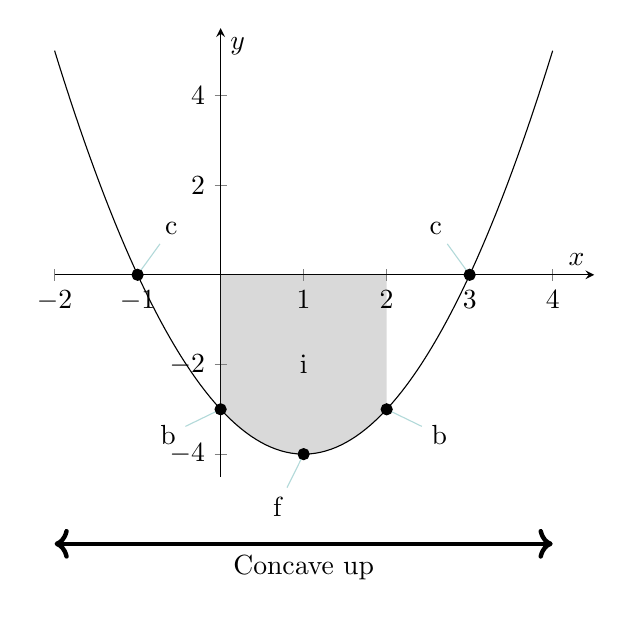
\begin{tikzpicture}
					\pgfplotsset{compat=1.12}
					\begin{axis}[xmin=-2, xmax=4.5, ymin=-4.5, ymax=5.5, xlabel={$x$}, ylabel={$y$}, axis lines = middle, samples=100, clip=false]
					% use TeX as calculator:
					\addplot[domain=-2:4,no markers,name path=f]{x^2-2*x-3};
					\path[name path=axis] (axis cs:0,0) -- (axis cs:2,0);
					\addplot[, fill=gray, fill opacity=0.3]
					fill between[
					of=f and axis,
					soft clip={domain=0:2},
					];
					
					\addplot[only marks] coordinates{(0,-3) (2,-3) (-1,0) (3,0) (1,-4)};
					\node[coordinate,pin=-170:{b}] at (axis cs:0,-3) {};
					\node[coordinate,pin=60:{c}] at (axis cs:-1,0) {};
					\node[coordinate,pin=120:{c}] at (axis cs:3,0) {};
					\node[coordinate,pin=-110:{f}] at (axis cs:1,-4) {};
					%\node[coordinate,pin=60:{f - max}] at (axis cs:1,2) {};
					\node[coordinate,pin=-10:{b}] at (axis cs:2,-3) {};
					\node[] at (axis cs:1,-2) {i};
					
					\draw[<->,ultra thick] (-2,-6) -- (4,-6) node[midway,below]{Concave up};
					%\draw[<-,ultra thick] (0,-4) -- (2,-4) node[midway,below]{Concave down};
					\end{axis}
					\end{tikzpicture}
				\end{center}
			\end{solution}
			
			\part Calculate the volume created when the area between $y=f(x)$ and $y=0$ from $x=0$ to $x=1$ is rotated about the $x$-axis.
			\begin{solution}
				\begin{align*}
					V &= \pi \int_0^1 y^2 \diffd x\\
					&= \pi \int_0^1 \left(x^2 - 2x - 3\right)^2 \diffd x\\
					&= \pi \int_0^1 x^4 - 2x^3 - 3x^2 -2x^3 + 4x^2 + 6x -3x^2 + 6x + 9 \diffd x \\
					&= \pi \int_0^1 x^4 - 4x^3 - 2x^2 + 12x + 9 \diffd x \\
					&= \pi \left[\frac{x^{5}}{5} - x^4 - \frac{2x^3}{3} + 6x^2 + 9x \right]_0^1 \\
					&= \pi \left[\left(\frac{1^{5}}{5} - 1^4 - \frac{2\cdot 1^3}{3} + 6 \cdot 1^2 + 9 \cdot 1 \right) - \left(\frac{0^{5}}{5} - 0^4 - \frac{2 \cdot 0^3}{3} + 6 \cdot 0^2 + 9 \cdot 0 \right)\right]\\
					&= \pi \left(\frac{1}{5} - 1 - \frac{2}{3} + 6 + 9\right)\\
					&= \frac{1 \cdot 3 - 3 \cdot 5 - 2 \cdot 5 + 6 \cdot 3 \cdot 5 + 9 \cdot 3 \cdot 5}{3 \cdot 5} \pi \\
					&= \frac{3 - 15  - 10 + 90 + 135}{15} \pi \\
					&= \uuline{\frac{203}{15} \pi \approx 42.52}
				\end{align*}
			\end{solution}
			
		\end{parts}
		\newpage
		%\vspace{2cm}
		\question
		A right angled triangle $ABC$ with side lengths $a$, $b$ and $c$  is shown in the figure.
		
		\begin{center}
			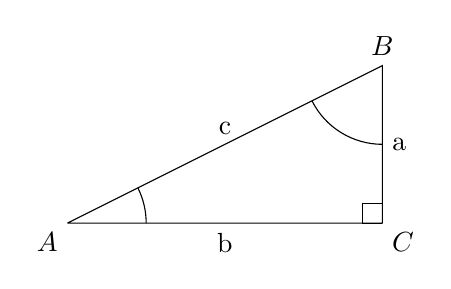
\begin{tikzpicture}
			
			\coordinate [label={below left:$A$}] (A) at (0,0);
			%\coordinate [label={below right:$A'$}] (A2) at (4,0);
			\coordinate [label={below right:$C$}] (C) at (4,0);
			\coordinate [label={above:$B$}] (B) at (4,2);
			
			\draw (A) -- node[above] {c}   (B) -- node[right] {a} (C) -- node[below] {b} (A);
			%\draw[dashed] (A2) -- node[right] {4} (B) -- (C) --  (A2);
			\tkzMarkRightAngle(B,C,A)
			\tkzMarkAngle(A,B,C)
			\tkzMarkAngle(C,A,B)
			%\node[below] at (C) {4};
			%\draw[thick] (0.4,0.0256) -- (0.4,1) -- (1,1);
			%\draw[decorate, decoration = {snake, amplitude = 0.3mm, segment length = 5.8mm}] (0.4,0.6) -- (0.88,0.6);
			%\draw[dashed] (0,1) -- (0.4,1);
			%\draw (0.88,0.6) -- (0.93, 0.6);
			%\draw[<->] (0.9,0) -- node[right] {$h$} (0.9,0.6);
			
			\end{tikzpicture}
		\end{center}
		\begin{parts}
			\part By expressing side $a$ and $b$ in terms of side $c$ and angle $A$, show that \[\sin^2 A + \cos^2 A = 1\] for $c>0$. The notation $\sin^2 A$ is equivalent to $\left(\sin A \right)^2$.
			
			\begin{solution}
				
				\begin{align*}
					\sin A &= \frac{a}{c} \Rightarrow a = c \sin A\\
					\cos A &= \frac{b}{c} \Rightarrow b = c \cos A\\
					\\
					a^2 + b^2 &= c^2\\
					c^2 \sin^2 A + c^2 \cos^2 A &= c^2\\
					\sin^2 A + \cos^2 A &= 1
				\end{align*}
			\end{solution}
			
			\part Given that $\sin A = 0.5$, determine $\cos A$ and $\tan B$.
			\begin{solution}
				We use the equation from (a) to find:
				\begin{align*}
					\sin^2 A + \cos^2 A &= 1\\
					\cos^2 A &= 1 - \sin^2 A\\
					\cos A &= \sqrt{1-\sin^2 A} = \sqrt{1-0.5^2} = \uuline{0.866}
				\end{align*}
				
				We can use the definition for tangent and the expressions we found for each side in (a):
				\begin{align*}
					\tan B &= \frac{b}{a} \\
					&= \frac{c \cos A}{c \sin A}\\
					&= \frac{\cos A}{\sin A}\\
					&= \frac{0.866}{0.5} = \uuline{1.73}
				\end{align*}
				
			\end{solution}
			
		\uplevel{The function
			\[f(t) = 0.25\cos(0.8 t )\]
			represents the fluctuations of water level in meters relative to mean level when waves are passing a specific point. $t$ is the time in seconds. A positive value of $f(t)$ means that the water level is higher than mean.
			
			}
		
			\part Determine the amplitude, period and frequency of the waves.
			
			\begin{solution}
				The amplitude is the coefficient of the cosine function, \uuline{$A=0.25$}. The angular frequency is the coefficient of time in the argument to the cosine function, $\omega = 0.8$. From this we find the frequency as \[f = \frac{\omega}{2 \pi} =\frac{0.8\, \mathrm{rad/s}}{2 \pi \, \mathrm{rad}} = \uuline{0.127 \,\mathrm{Hz}}\] and the period as \[T=\frac{1}{f}=\frac{1}{0.127 \, \mathrm{Hz}}=\uuline{\SI{7.85}{\second}}\]
			\end{solution}
			
			\part For $0 < t < T$, where $T$ is the period of the function $f(t)$, find the time $t$ when the water level is \SI{0.25}{\meter} below mean water level.
			
			\begin{solution}
				\begin{center}
					\begin{align*}
						f(t) &= -0.25\\
						0.25 \cos\left(0.8t\right) &= -0.25 \\
						\cos\left(0.8t\right) &= -1 \qquad \text{Only one solution for } 0<t<T\\
						0.8t &= \cos^{-1} \left(-1\right)\\
						0.8t &= \pi \\
						t &= \frac{\pi}{0.8} \approx \uuline{3.93}\\
						(t&=T/2)
					\end{align*}
					

				\end{center}
				
			\end{solution}
		\end{parts}

		\newpage
		\question
		The figure below shows four forces acting on the tip of a crane boom as a result of a hanging load. We do not consider the gravitational forces on the boom and on the wires. $F_1$ is the force from the hanging load, $F_2$ is the force from the wire holding the load, $F_3$ is the force from the wire holding the boom and $F_4$ is the force acting through the boom. The forces are given in component form, with unit \si{\kilo\newton}.
		
		
		
		\pgfdeclarelayer{back}
		\pgfsetlayers{back,main}
		
		\def\iangle{45}
		\def\arcr{1cm}
		
		\begin{center}
			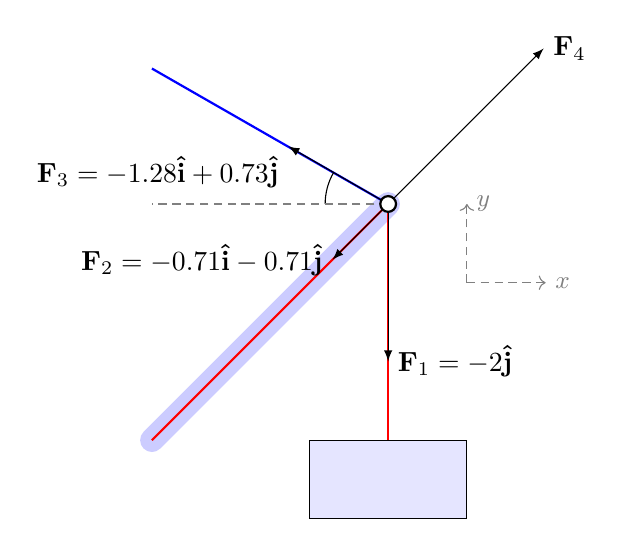
\begin{tikzpicture}[
			force/.style={>=latex,draw=black,fill=black},
			axis/.style={densely dashed,gray,font=\small},
			plane/.style={draw=black,fill=blue!10},
			string/.style={draw=red, thick},
			boom/.style={draw=gray, thick},
			ring/.style={thick, fill=white}, scale = 1
			]
			%\pgfmathsetmacro\ringy{tan(90-\iangle)}
			
			\coordinate (ring) at (0,0);
			\coordinate (load) at (0,-3);
			\coordinate (boombase) at (-3,-3);
			\coordinate (masttop) at (-3,1.72);
			
			%% Sketch
			\draw[plane] (load) -- ++(1,0) -- ++(0,-1) -- ++(-2,0) -- ++(0,1) -- cycle;
			%-- (0,1) coordinate (topleft)
			%-- coordinate[pos=0.5] (topmid) (2,1) coordinate (topright)
			%|- (base) -- cycle;
			%\node at (1,0.5) {God Jul!};
			
			
			
			%\begin{pgfonlayer}{back}
			\draw[line width=0.3cm,line cap=round,blue,opacity=0.2] (boombase) -- (ring);
			\draw[string] (load) -- (ring);
			\draw[string] (boombase) -- (ring);
			\draw[string, draw=blue] (ring) -- (masttop);
			%\draw[axis] (topmid) -- (ring);
			%\end{pgfonlayer}
			
			\draw[force, ->] (ring) -- ++(-90:2) node[right] {$\mathbf{F}_1 = -2\jvec$};
			\draw[force, ->] (ring) -- ++(-135:1) node[left] {$\mathbf{F}_2 = -0.71 \ivec -0.71 \jvec  $};
			\draw[force, ->] (ring) -- ++(-1.2679,0.732) node[below left] {$\mathbf{F}_3 = -1.28\ivec + 0.73\jvec$};
			\draw[force, ->] (ring) -- ++(1.975,1.975) node[right] {$\mathbf{F}_4$};% = 1.98\ivec + 1.98\jvec$};
			
			\coordinate (myxmin) at (-3,0);
			\tkzMarkAngle[label=$\alpha$, size=0.8](masttop,ring,myxmin)
			\draw[axis] (ring) -- (myxmin);
			
			\draw[axis, ->] (ring)++(1,-1) -- ++(1,0) node[right] {$x$};
			\draw[axis, ->] (ring)++(1,-1) -- ++(0,1) node[right] {$y$};
			
			\draw[ring] (ring) circle (0.1cm);
			
			%\draw (ring)++(0,-\arcr) arc (-90:\iangle-90:\arcr) node[midway,below]{$\iangle^\circ$};
			
			
			\end{tikzpicture}
		\end{center}
		\begin{parts}
			
			\part Determine the magnitude of $\mathbf{F}_3$ and the angle $\alpha$ between $\mathbf{F}_3$ and negative x-direction.
			\begin{solution}
				\begin{align*}
				F_3 &= \sqrt{x_3^2 + y_3^2} = \sqrt{\left(-1.28\right)^2 + \left(0.73\right)^2} = \uuline{1.47}\\
				\alpha &= \tan^{-1} \frac{0.73}{1.28} =\uuline{ \ang{29.7} = \SI{0.518}{\radian}}
				\end{align*}
			\end{solution}
			
			\part 
			The sum of the four forces is zero, determine the components of $\mathbf{F}_4$
			\begin{solution}
				\begin{align*}
					\mathbf{F}_1 + \mathbf{F}_2 + \mathbf{F}_3 + \mathbf{F}_4 &= 0  \\
					\mathbf{F}_4 &=  0 - \mathbf{F}_1 - \mathbf{F}_2 - \mathbf{F}_3 \\
					\mathbf{F}_4 &=  0 - \left(-2 \jvec \right) - \left( -0.71 \ivec -0.71 \jvec \right) - \left( -1.28\ivec + 0.73 \jvec\right) \\
					\mathbf{F}_4 &=  2 \jvec +0.71 \ivec +0.71 \jvec  +1.28\ivec - 0.73 \jvec \\
					\mathbf{F}_4 &=  \left(0.71 + 1.28\right) \ivec + \left(2 +0.71- 0.73\right) \jvec \\
					\mathbf{F}_4 &=  \uuline{1.99 \ivec + 1.98 \jvec} \\
				\end{align*}
	
			\end{solution}

			\part We change vertical component of the load force, $\mathbf{F}_1$, without changing the angle of the boom. In this case, all the forces changes proportionally to the load force. Determine the new value of the components of $\mathbf{F}_3$ if we change the load so that $\mathbf{F}_1 = -3\jvec$.
			
			\begin{solution}
				We first find the constants of proportionality from the original values
				\begin{align*}
					x_3 &= b_x x_1 \Rightarrow b_x = \frac{x_3}{x_1} = \frac{-1.28}{-2} = 0.64\\
					y_3 &= b_y x_1 \Rightarrow b_y = \frac{y_3}{x_1} = \frac{0.73}{-2} = -0.365\\
				\end{align*}
				Then we can use the constants of proportionality to determine the new values of the components of $\mathbf{F}_3$:
				\begin{align*}
					x_3 &= b_x x_1 = 0.64 \cdot (-3) = -1.92 \\
					y_3 &= b_y x_1 = -0.365 \cdot (-3) = 1.095 \approx 1.10 
				\end{align*}
				The new value of $\mathbf{F}_3$ is $\uuline{-1.92 \ivec + 1.10 \jvec}$.
			\end{solution}
		\end{parts}

		\vspace{12pt}
\newpage
		\question
		
		On a car ferry we count the number of persons per car:
		\begin{center}
			2 - 1 - 2 - 4 - 3 - 2 - 1 - 2 - 3 - 4 - 3 - 2 - 3 - 1 - 1 - 2 - 4 - 2 - 2 - 3
		\end{center}
		
		
		\begin{parts}
			\part Make a table of the frequency distribution.
			\begin{solution}
				\begin{center}
					\begin{tabular}{cc}
						\hline
						Passengers & Frequency\\
						\hline
						1 & 4 \\
						2 & 8 \\
						3 & 5 \\
						4 & 3 \\
						\hline
					\end{tabular}
				\end{center}
			\end{solution}

			
			\part Find the arithmetic mean, the mode and the median of the data set.
			\begin{solution}
				We can make use of the frequency distribution to make the calculation of the arithmetic mean faster:
				\[\bar{x} = \frac{\sum_{i=1}^{4}x_i f_i}{\sum_{i=1}^{4}f_i}=\frac{1\cdot4 + 2\cdot8 + 3\cdot5 +4\cdot3}{5+8+5+3}=\frac{48}{20} = \uuline{2.35}\]
				
				The \uline{mode} is the most frequently occurring number of passengers, \uuline{2} passengers.
				The median is the middle in the ordered set, or in this case the average of value 10 and 11. Both number 10 and 11 is 2, so the \uuline{median is 2}.
			\end{solution}
			
			\uplevel{By counting the number of passengers per car over a month, we found the following probability distribution:
			\vspace{3pt}
			\begin{center}
				\begin{tabular}{cc}
					\hline
					Passengers & Probability\\
					\hline
					1 & 0.30 \\
					2 & 0.35 \\
					3 & 0.20 \\
					4 & 0.15 \\
					\hline
				\end{tabular}
			\end{center}
			\vspace{12pt}
			
			We select two random cars and define the following events:
			
			\begin{description}
				\item[$E_1$] The two cars have 3 persons each
				\item[$E_2$] One of the two cars has 2 persons, the other has 4 persons.
				\item[$E_3$] The two cars have 6 persons in total
				\item[$E_4$] The two cars have 5 or fewer persons in total
				\item[$E_5$] The two cars have 6 or more persons in total
			\end{description}}
			
			\vspace{5pt}
				
			\part Which events are mutually exclusive and which are complementary?
			\begin{solution}
				Mutually exclusive are:\\ 
				\uuline{$E_1$, $E_2$ and $E_4$}\\
				\uuline{$E_3$ and $E_4$}\\
				\uuline{$E_4$ and $E_5$}\\
				Alternatively this is written as $E_1$ and $E_2$, $E_1$ and $E_4$, $E_2$ and $E_4$, $E_3$ and $E_4$, $E_4$ and $E_5$. %The events that are not mutually exclusive are $E_1$ and $E_3$, and $E_2$ and $E_3$.\\
				Complementary events are:\\
				\uuline{$E_4$ and $E_5$}
			\end{solution}
			
			\part Determine the two probabilities $P(E_1)$ and $P(E_2)$.
			\begin{solution}
				$E_1$ can only occur in one way, that both cars have 3 persons. We use the multiplication law for independent events (the number of persons in the second car is independent of the number of persons in the first car).
				\[P(E_1) = P(x=3)\cdot P(x=3) = 0.20 \cdot 0.20 = \uuline{0.04}\]
				
				$E_2$ can occur in 2 different ways; 2 persons in the first car and 4 in the second car or 4 persons in the first car and 2 in the second.
				\begin{align*}
					P(E_2) &= P(x=2)P(x=4) + P(x=4)P(x=2) \\
					P(E_2) &= 0.35\cdot 0.15 + 0.15 \cdot 0.35 = \uuline{0.105}
				\end{align*}
			\end{solution}
			
			\part Determine the two probabilities $P(\overline{E_1})$ and $P(\overline{E_4})$.
			\begin{solution}
				We already know $P(E_1)$, so
				\[P(\bar{E}_1) = 1- P(E_1)=1-0.04=\uuline{0.96}\]
				Since $E_4$ is complementary to $E_5$, $P(\bar{E}_4) = P(E_5)$. $E_5$ can occur in six different ways; 2+4, 3+3, 3+4, 4+2, 4+3, 4+4.
				 
				\begin{align*}
					P(\bar{E}_4) &= P(x=2)P(x=4) + P(x=3)P(x=3) + P(x=3)P(x=4) +\\
					 &\qquad P(x=4)P(x=2) + P(x=4)P(x=3) + P(x=4)P(x=4)\\
					P(\bar{E}_4) &= 0.35 \cdot 0.15 + 0.2 \cdot 0.2 + 0.2 \cdot 0.15 + 0.15 \cdot 0.35 + 0.15 \cdot 0.2 + 0.15 \cdot 0.15 \\
					P(\bar{E}_4) &= \uuline{0.2275}
				\end{align*}
			\end{solution}
			
			\part Determine $P(E_4 | E_5)$ and $P(E_3|E_1)$.
			
			\begin{solution}
				(In some sense this is a trick question, testing the understanding of conditional probability. Only logical reasoning is needed, no calculations.)
				
				$P(E_4 | E_3)$ we know that the cars have 6 or more persons in total, then they can not have 5 or less persons in total
				\[\uuline{P(E_4 | E_5) = 0}\]
				
				$P(E_3 | E_1)$ we know that the cars have 3 persons each, so we can be sure that they have 6 persons in total
				\[\uuline{P(E_3 | E_1) = 1}\]
			\end{solution}
			
		\end{parts}
		
		
	\end{questions}
	
	\newpage
	
	\include{formulasheet}
	
\end{document} 
